\chapter[Hall A Vacuum System]{Hall A Vacuum System
\label{chap:vacuum}
\footnote{
  $CVS~revision~ $Id: vacuum.tex,v 1.4 2005/04/04 22:27:25 gen Exp $ $ 
}
\footnote{Authors: J.LeRose \email{lerose@jlab.org}}
}
\section{Overview}

The Hall A vacuum system consists of 5 separate but interconnected 
subsystems.  The largest is designed to supply 
the Hall A HRS (see Chapter \ref{chap:hrs}) with a 
self contained 5 $\times$ 10$^{-6}$ Torr vacuum that enables both 
spectrometers to be pumped down from atm. in a few hours.  The target 
vacuum system is designed to maintain a 1 $\times$ 10$^{-6}$ Torr in 
order to minimize contamination and provide an insulating vacuum for the 
cryo target.  Rough insulating vacuum for the 4 superconducting magnets 
is provided by a 360 $cfm$ Roots type blower that can be connected to each 
magnet.  The beam line vacuum is maintained by 1 $\ell$/s ion pump 
system used in the accelerator ring and a small turbo pump located near 
the target.  The final subsystem is a differential pumping station 
located near the target exit port.

\infolevone{
\section{HRS Vacuum System}

The HRS vacuum system is shown in Figure~\ref{fig:hrs_vac_sys}.
Vacuum for the HRS is supplied by an Alcatel 880 $\ell$/s Turbo 
pump backed by a Balzers 360 $cfm$ Roots type Blower.  This Blower, via a 
special manifold, also supplies the roughing vacuum to the HRS at the 
Dipole Inlet Transition.  The first Turbo is mounted on the lower side 
of the Dipole entrance transition.  The roughing port is also located on 
this transition, on the top side.  The upper turbo is located on the 
lower side of the window transition.

Vacuum readouts and interlock outputs are supplied by five (5) HPS 
series 421 Cold Cathode gauges and seven (7) series 275 Mini-Convectron 
gauges.  In addition to these there will also be a FIsons Micromass 386 
RGA head installed in the system for diagnostic purposes.  Most of this 
instrumentation will be located on the Turbo pump manifold (for detailed 
information see Figure~\ref{fig:hrs_vac_sys}).

\begin{figure}
\begin{center}
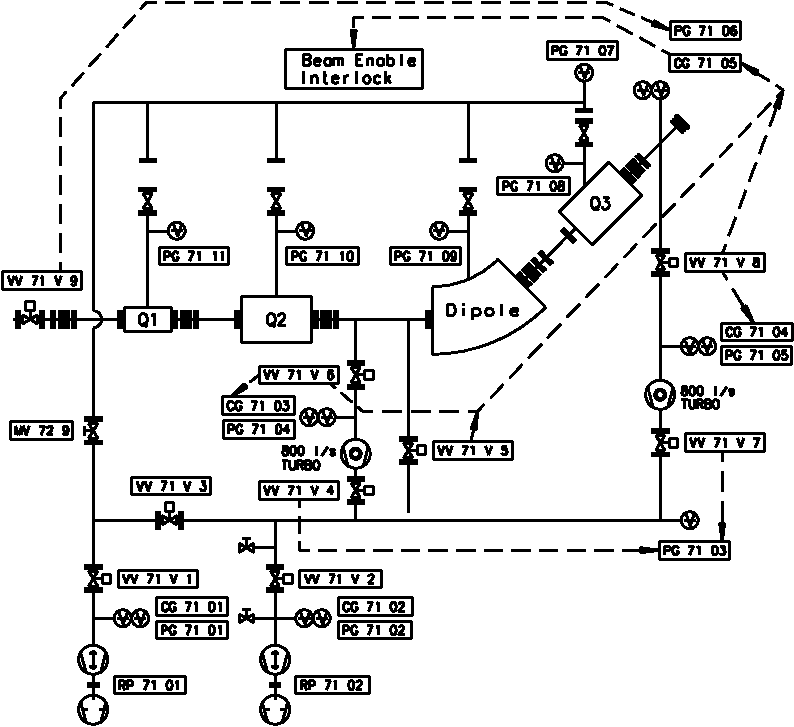
\includegraphics[angle=0,width=15cm]{fig0125new}
{\linespread{1.}
\caption[Spectrometers: HRS Vacuum System]{HRS vacuum system.}
\label{fig:hrs_vac_sys}}
\end{center}
\end{figure}

Powered valves, instrumentation and pumps will be controlled and powered 
at the Vacuum System equipment rack located on each respective 
spectrometer on the gantry platform.  Selective equipment will also be 
controllable from the Hall A counting house.

{\bf Chamber}

The HRS vacuum chamber consists of an associated vacuum window, a sieve 
slit and Q1 transition, Q1 to Q2 transition, Spool section, Dipole 
transition, Dipole to Q3 transition, and the Q3 to exit window assembly. 
 The spectrometer vacuum is contained by a 0.007 inch kapton window at the
 entrance and a 0.004 inch titanium window at the exit.

\section{Target Vacuum System}

Vacuum for the target chamber is supplied by an Alcatell 880 $\ell$/s 
Turbo pump backed by an Alcatell 21 $cfm$ 2 stage vane pump.  The Turbo is 
mounted on the lower ring of the Target Chamber to one side so as not to 
interfere with the Target Chamber windows.

The same instrumentation is used here as on the spectrometer.

Powered valves, instrumentation and pumps will be controlled and powered 
at the Vacuum System equipment rack located on the access Balcony.  
Selective equipment will also be controllable from the Hall A counting 
house. 

\section{Magnet Vacuum System}

Vacuum for the magnet insulating vacuum is provided by the Cryo
pumping effects of each individual magnet.

All controls for the Magnets are manual as we expect no problem after 
initial pump down.


The insulating vacuum for each magnet is self contained within the 
magnet.

\section{Beam Line Vacuum System}

Vacuum for the entrance beam line is supplied by 65 $\ell$/s Balzers turbo
pumps, the first of which is located on the E P chamber, and the
second located 3 $m$ upstream of the target chamber.  Both turbos
are equipped with a HPS 7 Series 275 mini Convectron gauge and a HPS
series 421 Cold Cathode gauge located near the balcony.

Vacuum readouts and relay outputs for interlocks are supplied by HPS series 421 
Cold Cathode gauges.  In addition to these there will also be Convectron 
gauges.  Most of this instrumentation will be located on the Turbo pump 
manifold.

Powered valves, instrumentation and pumps will be controlled and powered 
at the Vacuum System equipment rack located on the Balcony.  Selective 
equipment will also be monitored from the Hall A counting house.  All 
control is by Accelerator in the MCC.

\section{Beam Exit Vacuum System}

Vacuum for the target chamber is supplied by an Alcatell 880
$\ell$/s Turbo pump backed by an Alcatell 21 $cfm$ 2 stage vane pump
which maintains a $1x10^{-4}$ vacuum on the exit beam pipe.

Between the target chamber and the exit beam pipe there is a 0.007 inch
kapton window that has a 0.0375 inch hole in it at the beam spot.  This
window acts as a differential pumping station.

Also between the target chamber and the exit beam pipe is an 8 inch
air actuated gate valve that is operated from the MCC.

Vacuum readouts and interlocks outputs are supplied by an HPS 7 Series 
275 mini Convectron and an HPS series 421 Cold Cathode gauge
which are located near the balcony.

Controls are interlocked to the beam.

The chamber is made of a low mass aluminum corrugated vacuum tube of 1 
$m$ diameter.

At the exit point of the exit beam pipe is a beam diffuser that
consists of 2.025 inch beryllium windows with a water filled cavity between
them for cooling.  The water is circulated through the cavity by a
water cooling system located on the Hall floor, and is interlocked
through the FSD system with 2 flow switches, one on the supply and
one on the return line.

Due to high radiation levels at the exit beam pipe all seals in
this area are metal.
} %infolev

\begin{safetyen}{10}{15}
\section{Hazards of Vacuum Systems}
\end{safetyen}

Hazards associated with the vacuum system are due to rapid 
decompression in case of a window failure. Loud noise can cause hearing
loss.  To mitigate the hazard, all personnel in the vicinity of the 
large chamber with a window are required to wear ear protection when
the chamber is under vacuum. Warning signs must be posted at the area.

The scattering chamber is equipped with a large 0.016~$in$ aluminum window that 
allows the spectrometers to swing from 12.5$^{\circ}$ to 165$^{\circ}$ 
on the left side and 12.5$^{\circ}$ to 140$^{\circ}$ on the right side. 
In order to
protect this window when the Hall is open, lexan window guards are
installed.

At the inlet of the sieve slit a M{\o}ller 8" diameter 7 mil kapton window 
is provided to separate the target chamber from the spectrometers.

Finally, under the detectors, a 4 mil titanium window is provided.  

The 1 $\ell$/s vac ion and the cold cathode gauges operate at several 
KV; consequently there is also a shock hazard.

Additionally, all vacuum vessels and piping are designed as pressure 
vessels.

\infolevone{\newpage}
\begin{safetyen}{10}{15}
\section{Authorized Personnel}
\end{safetyen}
The authorized personnel is shown in Table \ref{tab:vacuum:personnel}.
\begin{namestab}{tab:vacuum:personnel}{Vacuum: authorized personnel}{%
      Vacuum in Hall A: authorized personnel. ''W.B'' stands for the white board 
      in the counting house.}
  \TechonCall{\em Contact}
  \EdFolts{}
\end{namestab}


